% !TEX root = handbook-physics.tex
% !TEX TS-program = pdflatex
% !TEX encoding = UTF-8 Unicode






\chapter[Motion of Charged Particles]{Motion Of Charged Particles In Electric And Magnetic Fields}
\label{ch-24}
\zhtitle{电场与磁场中带电粒子的运动}

\section{Lorentz Force}
\label{sec-24.1}
\zhtitle{洛伦兹力}

\begin{marginfigure}%[-2cm]
\centering
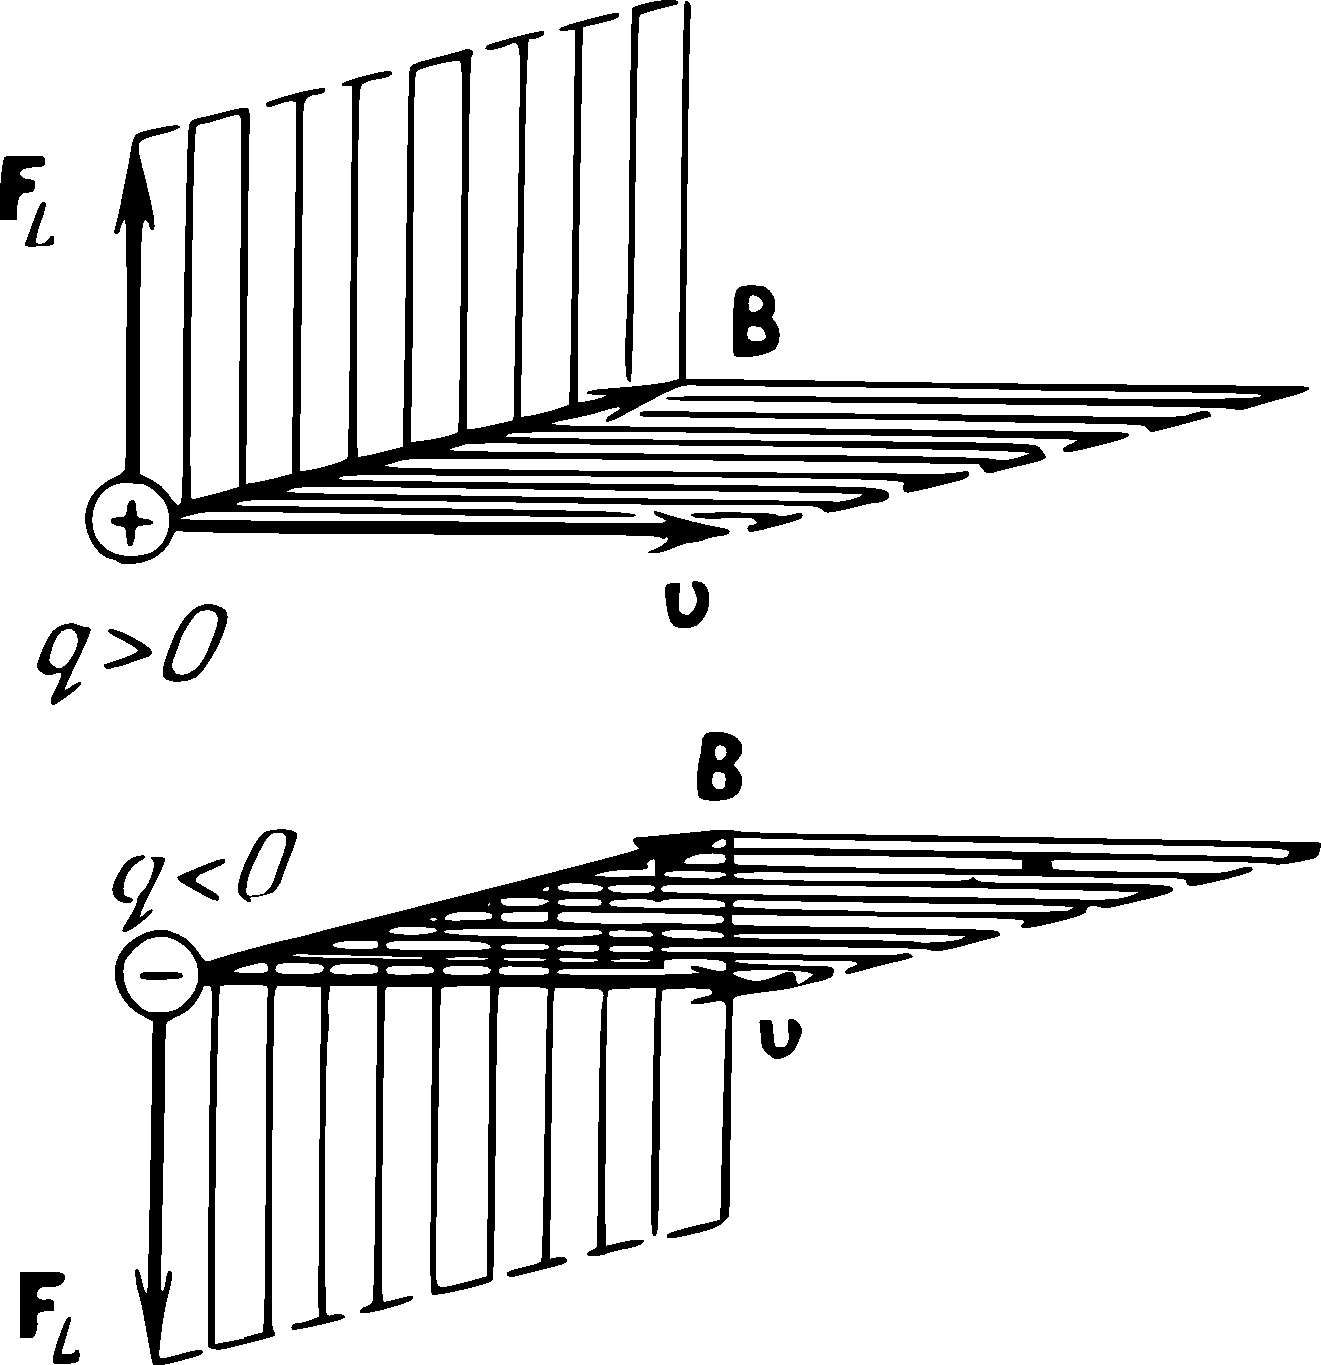
\includegraphics[width=0.9\textwidth]{figs/ch-24/fig-24-01.pdf}
\sidecaption{The relative arrangement of vectors $\vb{v}$, $\vb{B}$ and $\vb{F}_{L}$ for positive and negative charges.\zhcap{正、负电荷情形下矢量 $\vb{v}$、$\vb{B}$ 与 $\vb{F}_{L}$ 的相对排列。}\label{fig-24-01}}
\end{marginfigure}
\subsection{}\label{24.1.1} 

Not only current-carrying conductors \ssect{23.1.4} are subject to the action of a magnetic field. This is also true of separate charged particles moving in the field. The force $F_{L}$, acting on an electric charge $q$ moving in a magnetic field at the velocity $\vb{v}$, is called the \redem{Lorentz force} and is equal to (see also \ssect{24.1.5})
\zhpar{不仅载流导体（\ssect{23.1.4}）受磁场的作用，场中运动的单个带电粒子同样受磁场的作用。以速度 $\vb{v}$ 在磁场中运动的电荷 $q$ 所受的力 $F_{L}$ 称为\redem{洛伦兹力}（另见\ssect{24.1.5}），其大小由下式给出：}
\begin{align*}%
F_{L} & = q\,[\vb{v} \cross \vb{B}] &&  \text{(in SI units),} \\
F_{L} & = \frac{q}{c} [\vb{v} \cross \vb{B}] &&  \text{(in Gaussian units),}
\end{align*}
where $q$ is the algebraic value of the moving charge, $\vb{B}$ is the induction of the magnetic field in which the charge is moving \ssect{23.1.2}, and $c$ is the electrodynamic constant \ssect{23.2.2}. The relative arrangement of vectors $\vb{v}$, $\vb{B}$ and $\vb{F}_{L}$ is shown in \figr{fig-24-01} for positive $(q > 0)$ and negative $(q < 0)$ charges. The magnitude of the Lorentz force is
\zhpar{式中 $q$ 为运动电荷的代数值，$\vb{B}$ 为运动电荷所处磁场的磁感应强度（\ssect{23.1.2}），$c$ 为电动力学常量（\ssect{23.2.2}）。矢量 $\vb{v}$、$\vb{B}$ 与 $\vb{F}_{L}$ 的相对方向如\figr{fig-24-01}所示，分别针对正电荷（$q > 0$）和负电荷（$q < 0$）。洛伦兹力的大小为：}
\begin{equation*}%
F_{L} = qvB \sin \alpha,
\end{equation*}
where $\alpha$ is the angle between vectors $\vb{v}$ and $\vb{B}$.
\zhpar{式中 $\alpha$ 为矢量 $\vb{v}$ 与 $\vb{B}$ 之间的夹角。}



\subsection{}\label{24.1.2}

The Lorentz force is always perpendicular to the velocity of the charged particle and imparts normal acceleration \ssect{1.4.6} to it. Since the Lorentz force does not change the magnitude of the velocity, but only its direction, this force does no work and the kinetic energy of the charged particle remains constant when it moves in a magnetic field. 
\zhpar{洛伦兹力总是垂直于带电粒子的速度，并使其产生法向加速度（\ssect{1.4.6}）。由于洛伦兹力只改变速度的方向而不改变速度的大小，所以该力不做功，带电粒子在磁场中运动时其动能保持不变。}

\subsection{}\label{24.1.3}

Making use of the Lorentz force, magnetic induction $\vb{B}$ \ssect{23.1.2} can be defined as follows: the magnitude of the magnetic induction vector at a given point of the magnetic field is equal to the maximum Lorentz force $F_{L\,\text{max}}$ acting on a unit positive charge, which, at the given point, travels at unit velocity. Thus
\zhpar{利用洛伦兹力，可以如下定义磁感应强度 $\vb{B}$（\ssect{23.1.2}）：磁场中某点磁感应强度矢量的大小，等于在该点以单位速度运动的单位正电荷所受的最大洛伦兹力。于是有：}
\begin{equation*}%
B = \frac{F_{L\,\text{max}}}{qv}.
\end{equation*}
Here $F_{L} = F_{L\,\text{max}}$ under the condition that $\alpha = \pi/2$ \ssect{24.1.2}. See also Sections \ssect{23.1.2} and \ssect{23.4.2}.
\zhpar{此处 $F_{L} = F_{L\,\text{max}}$ 的条件为 $\alpha = \pi/2$（\ssect{24.1.2}）。另见 \ssect{23.1.2} 和 \ssect{23.4.2}。}

\subsection{}\label{24.1.4}

The force exerted on moving charge $q_{2}$ by moving charge axis called \redem{the force of their magnetic interaction} (\redem{magnetic force}). For the special case of two positive charges $q_{1}$ and $q_{2}$, travelling in vacuum at the same velocity $v_{1} = v_{2} = v \ll c$ along the $OX$ axis, the force $F_{\text{int}}$ of magnetic interaction is a force of attraction and is numerically equal to
\zhpar{运动电荷 $q_{2}$ 受到另一运动电荷作用的力，称为\redem{磁相互作用力}（\redem{磁力}）。对于真空中两个正电荷 $q_{1}$ 和 $q_{2}$ 以相同速度 $v_{1} = v_{2} = v \ll c$ 沿 $OX$ 轴运动的特殊情形，其磁相互作用力 $F_{\text{int}}$ 为吸引力，数值上等于：}
\begin{equation*}%
F_{\text{int}} = \frac{\mu_{0}}{4 \pi}\, \frac{q_{1}q_{2}}{r^{2}} v^{2} \,\, \text{(in SI units)},
\end{equation*}
where $r$ is the distance between the charges, and $\mu_{0}$ is the magnetic constant \ssect{23.2.2}.
\zhpar{式中 $r$ 为两电荷之间的距离，$\mu_{0}$ 为磁常量（\ssect{23.2.2}）。}

The force $F_{\text{int}}$ of magnetic interaction can be presented in the form
\zhpar{磁相互作用力 $F_{\text{int}}$ 也可以写成如下形式：}
\begin{equation*}%
F_{\text{int}} = q_{2}v\, \frac{\mu_{0}q_{1}v}{4 \pi r^{2}} = q_{2}vB,
\end{equation*}
where
\zhpar{式中：}
\begin{equation*}%
B = \frac{\mu_{0}q_{1}v}{4 \pi r^{2}}.
\end{equation*}
In this form the force $F_{\text{int}}$ coincides with the Lorentz force at $\sin \alpha = l$ \ssect{24.1.1} if we assume that $B$ is the induction of the magnetic field \ssect{23.1.2} set up by moving charge $q_{1}$. In its turn, this field acts on moving charge $q_{2}$. Magnetic forces and a magnetic field are the result of the way in which forces are transformed in going over from a fixed to a moving frame of reference, and follows from the formulas of the special theory of relativity \ssect{5.1.1}.
\zhpar{在这种形式下，若假定 $B$ 为电荷 $q_{1}$ 所产生的磁场的磁感应强度（\ssect{23.1.2}），则当 $\sin \alpha = l$（\ssect{24.1.1}）时，力 $F_{\text{int}}$ 与洛伦兹力一致。该磁场又作用于运动电荷 $q_{2}$。磁力和磁场是力在静止参考系与运动参考系之间变换的结果，可由狭义相对论的公式（\ssect{5.1.1}）导出。}

Comparing force $F_{\text{int}}$ with the force $F_{e}$ of electrostatic repulsion between mutually fixed charges $q_{1}$ and $q_{2}$ in vacuum $(\varepsilon_{r} = 1)$ located at the same distance $r$ from each other \ssect{14.2.6}
\zhpar{将磁相互作用力 $F_{\text{int}}$ 与真空中（$\varepsilon_{r} = 1$）位于同一距离 $r$ 处、彼此固定的电荷 $q_{1}$、$q_{2}$ 之间的静电斥力 $F_{e}$（\ssect{14.2.6}）相比较，有：}
\begin{equation*}%
F_{e} = \ofpe \frac{q_{1}q_{2}}{r^{2}}\,\, \text{(in SI units)},
\end{equation*}
where $\varepsilon_{0}$ is the electric constant in SI units), we readily find that
\zhpar{式中 $\varepsilon_{0}$ 为电常量（SI 单位制中的真空电容率），由此可以很容易地得到：}
\begin{equation*}%
\frac{F_{\text{int}}}{F_{e}} =\frac{v^{2}}{c^{2}},
\end{equation*}
where $c$ is the electrodynamic constant \ssect{23.2.2} and is related to $\varepsilon_{0}$ and $\mu_{0}$ by the equation $\varepsilon_{0}\mu_{0}= 1/c^{2}$ (Appendix~I). When the velocity of the charges is small compared to the velocity of light in free space $(v \ll c)$, the magnetic interaction between the moving charges is considerably less than their electrostatic interaction. But in the case when the charges are moving in an electrically neutral conductor, the electric forces are compensated \ssect{16.4.2}, leaving only magnetic interaction. This explains the magnetic interaction of current-carrying conductors \ssect{23.4.1}. Though the force of magnetic interaction between each pair of electrons is small, the number of pairs is so immense that the resultant force of magnetic interaction of parallel current-carrying conductors is an appreciable amount \ssect{23.4.1}.
\zhpar{式中 $c$ 为电动力学常量（\ssect{23.2.2}），它与 $\varepsilon_{0}$、$\mu_{0}$ 的关系为 $\varepsilon_{0}\mu_{0}= 1/c^{2}$（附录~I）。当电荷的速度远小于真空中的光速（$v \ll c$）时，运动电荷之间的磁相互作用远小于它们之间的静电相互作用。但当电荷在电中性导体中运动时，电场力相互抵消（\ssect{16.4.2}），只剩下磁相互作用。这就解释了载流导体之间的磁相互作用（\ssect{23.4.1}）。虽然每一对电子之间的磁相互作用很小，但电子对的数目极其巨大，因此平行载流导体之间的合磁相互作用力是相当可观的（\ssect{23.4.1}）。}

\subsection{}\label{24.1.5} If, in addition to a magnetic field of induction $\vb{B}$, a moving electric charge is also subject to the action of an electric field of strength $\vb{E}$ \ssect{15.1.2}, the resultant force $\vb{F}$ applied to the charge is equal to the vector sum of the force $\vb{F}_{e} = q\vb{E}$, exerted on the charge by the electric field and the Lorentz force \ssect{24.1.1}t
\zhpar{若运动的电荷除受磁感应强度为 $\vb{B}$ 的磁场作用外，还受到电场强度为 $\vb{E}$ 的电场作用（\ssect{15.1.2}），则作用于电荷的合力 $\vb{F}$ 等于电场对电荷的作用力 $\vb{F}_{e} = q\vb{E}$ 与洛伦兹力（\ssect{24.1.1}）的矢量和，即：}
\begin{align*}%
\vb{F} & = q\,\vb{E} + q\,[\vb{v} \cross \vb{B}]  &&  \text{(in SI units),} \\
\vb{F} & = q\,\vb{E} + \frac{q}{c}\,[\vb{v} \cross \vb{B}]  &&  \text{(in Gaussian units),}
\end{align*}
The last expression is also called the Lorentz force and, sometimes, the \redem{generalized Lorentz force} or the \redem{Lorentz formula}. 
\zhpar{上式也称为洛伦兹力，有时亦称为\redem{广义洛伦兹力}或\redem{洛伦兹公式}。}

\subsection{}\label{24.1.6} By the action of the Lorentz force \ssect{24.1.1}, a charged particle travels in a circular path of constant radius $r$ in a uniform magnetic field perpendicular to the particle's velocity. This circular path is in a plane perpendicular to vector $\vb{B}$, and the Lorentz force is a centripetal one \ssect{2.4.3}. The radius of the circular path is
\zhpar{在磁感应强度为 $\vb{B}$ 的均匀磁场中，若带电粒子的速度与磁场垂直，则洛伦兹力（\ssect{24.1.1}）使粒子沿半径恒为 $r$ 的圆轨道运动。该圆轨道位于与矢量 $\vb{B}$ 垂直的平面内，洛伦兹力即为向心力（\ssect{2.4.3}）。圆轨道的半径为：}
\begin{align*}%
r & = \frac{m}{\abs{q}} \,\frac{v}{B}  &&  \text{(in SI units),} \\
r & = \frac{cm}{\abs{q}} \, \frac{v}{B}   &&  \text{(in Gaussian units),}
\end{align*}
where $\abs{q}$ is the absolute value of the particle's charge, $m$ is the mass of the particle, $v$ is its velocity, $B$ is the magnetic field induction and $c$ is the electrodynamic constant \ssect{23.2.2}. If the particle travels in the plane of the drawing (\figr{fig-24-02}), its deflection in a field perpendicular to the velocity and directed from behind the drawing depends upon the sign of the charge. 
\zhpar{式中 $\abs{q}$ 为粒子电荷的绝对值，$m$ 为粒子的质量，$v$ 为其速度，$B$ 为磁感应强度，$c$ 为电动力学常量（\ssect{23.2.2}）。若粒子在图面内运动（见\figr{fig-24-02}），则其在与速度垂直、且自图面后方指向前方的磁场中的偏转方向取决于电荷的正负。}

This is the basis for determining the sign of the charge of a particle travelling in a magnetic field.
\zhpar{这正是判断在磁场中运动的粒子所带电荷正负的依据。}

\begin{marginfigure}[-3cm]
\centering
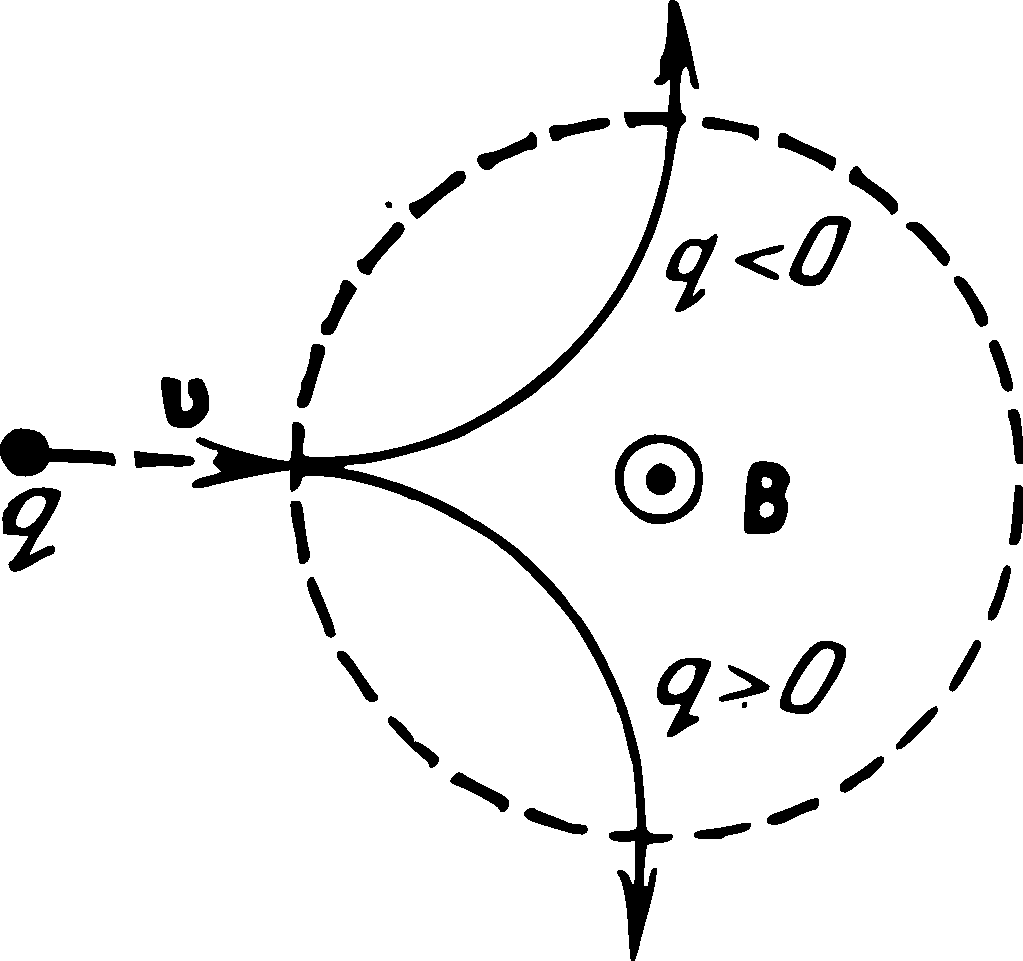
\includegraphics[width=0.8\textwidth]{figs/ch-24/fig-24-02.pdf}
\sidecaption{Path of a charged particle in a magnetic field depends on the sign of its charge.\zhcap{带电粒子在磁场中的轨迹取决于其电荷的正负。}\label{fig-24-02}}
\end{marginfigure}

The period $T$ of revolution \ssect{1.5.5} of a charged particle in a uniform magnetic field \ssect{23.1.3} is independent of its velocity (when $v \ll c$):
\zhpar{在均匀磁场（\ssect{23.1.3}）中运动的带电粒子，其回旋周期 $T$（\ssect{1.5.5}）与速度无关（当 $v \ll c$ 时）：}
\begin{align*}%
T & = \frac{2 \pi }{B}\,\frac{m}{\abs{q}}  &&  \text{(in SI units),} \\
r & = \frac{2 \pi }{B}\,\frac{mc}{\abs{q}}  &&  \text{(in Gaussian units),}
\end{align*}
The principle of cyclic orbit accelerators of charged particles \ssect{24.4.6} is based on the aforesaid.
\zhpar{带电粒子循环轨道加速器（\ssect{24.4.6}）的原理即以上述结论为基础。}


\begin{marginfigure}[1cm]
\centering
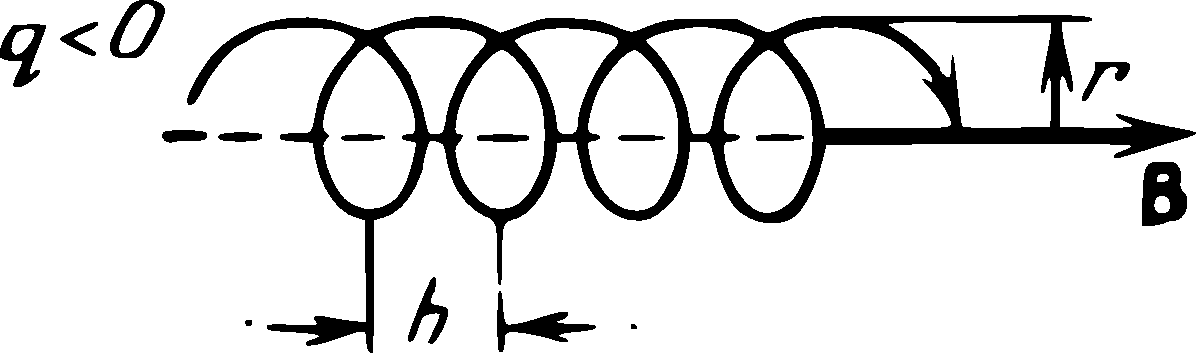
\includegraphics[width=0.8\textwidth]{figs/ch-24/fig-24-03.pdf}
\sidecaption{Path of a charged particle is a helix if the velocity vector $\vb{v}$ of a charged particle makes the angle $\alpha$ with the direction of vector $\vb{B}$ of a uniform magnetic field.\zhcap{若带电粒子的速度矢量 $\vb{v}$ 与均匀磁场的磁感应强度 $\vb{B}$ 方向成夹角 $\alpha$，则其轨迹为螺旋线。}\label{fig-24-03}}
\end{marginfigure}

\subsection{}\label{24.1.7} If the velocity vector $\vb{v}$ of a charged particle makes the angle $\alpha$ with the direction of vector $\vb{B}$ of a uniform magnetic field, the particle travels along a helix (\figr{fig-24-03}) of radius $r$ and pitch $h$ equal to
\zhpar{若带电粒子的速度矢量 $\vb{v}$ 与均匀磁场的磁感应强度 $\vb{B}$ 方向成夹角 $\alpha$，则粒子沿螺旋线运动（见\figr{fig-24-03}），螺旋线的半径 $r$ 与螺距 $h$ 分别为：}
\begin{alignat*}{3}%
r & = \frac{m}{\abs{q}} \,\frac{v \sin \alpha}{B},\,\, && h  = \frac{2 \pi}{B} \,\frac{m}{\abs{q}} \, v \cos \alpha \,\,&&  \text{(in SI units),} \\
r & =  \frac{mc}{\abs{q}} \,\frac{v \sin \alpha}{B}, \,\,&& h  = \frac{2 \pi}{B} \,\frac{mc}{\abs{q}} \, v \cos \alpha \,\,&&  \text{(in Gaussian units.)}
\end{alignat*}
\begin{marginfigure}[-1cm]
\centering
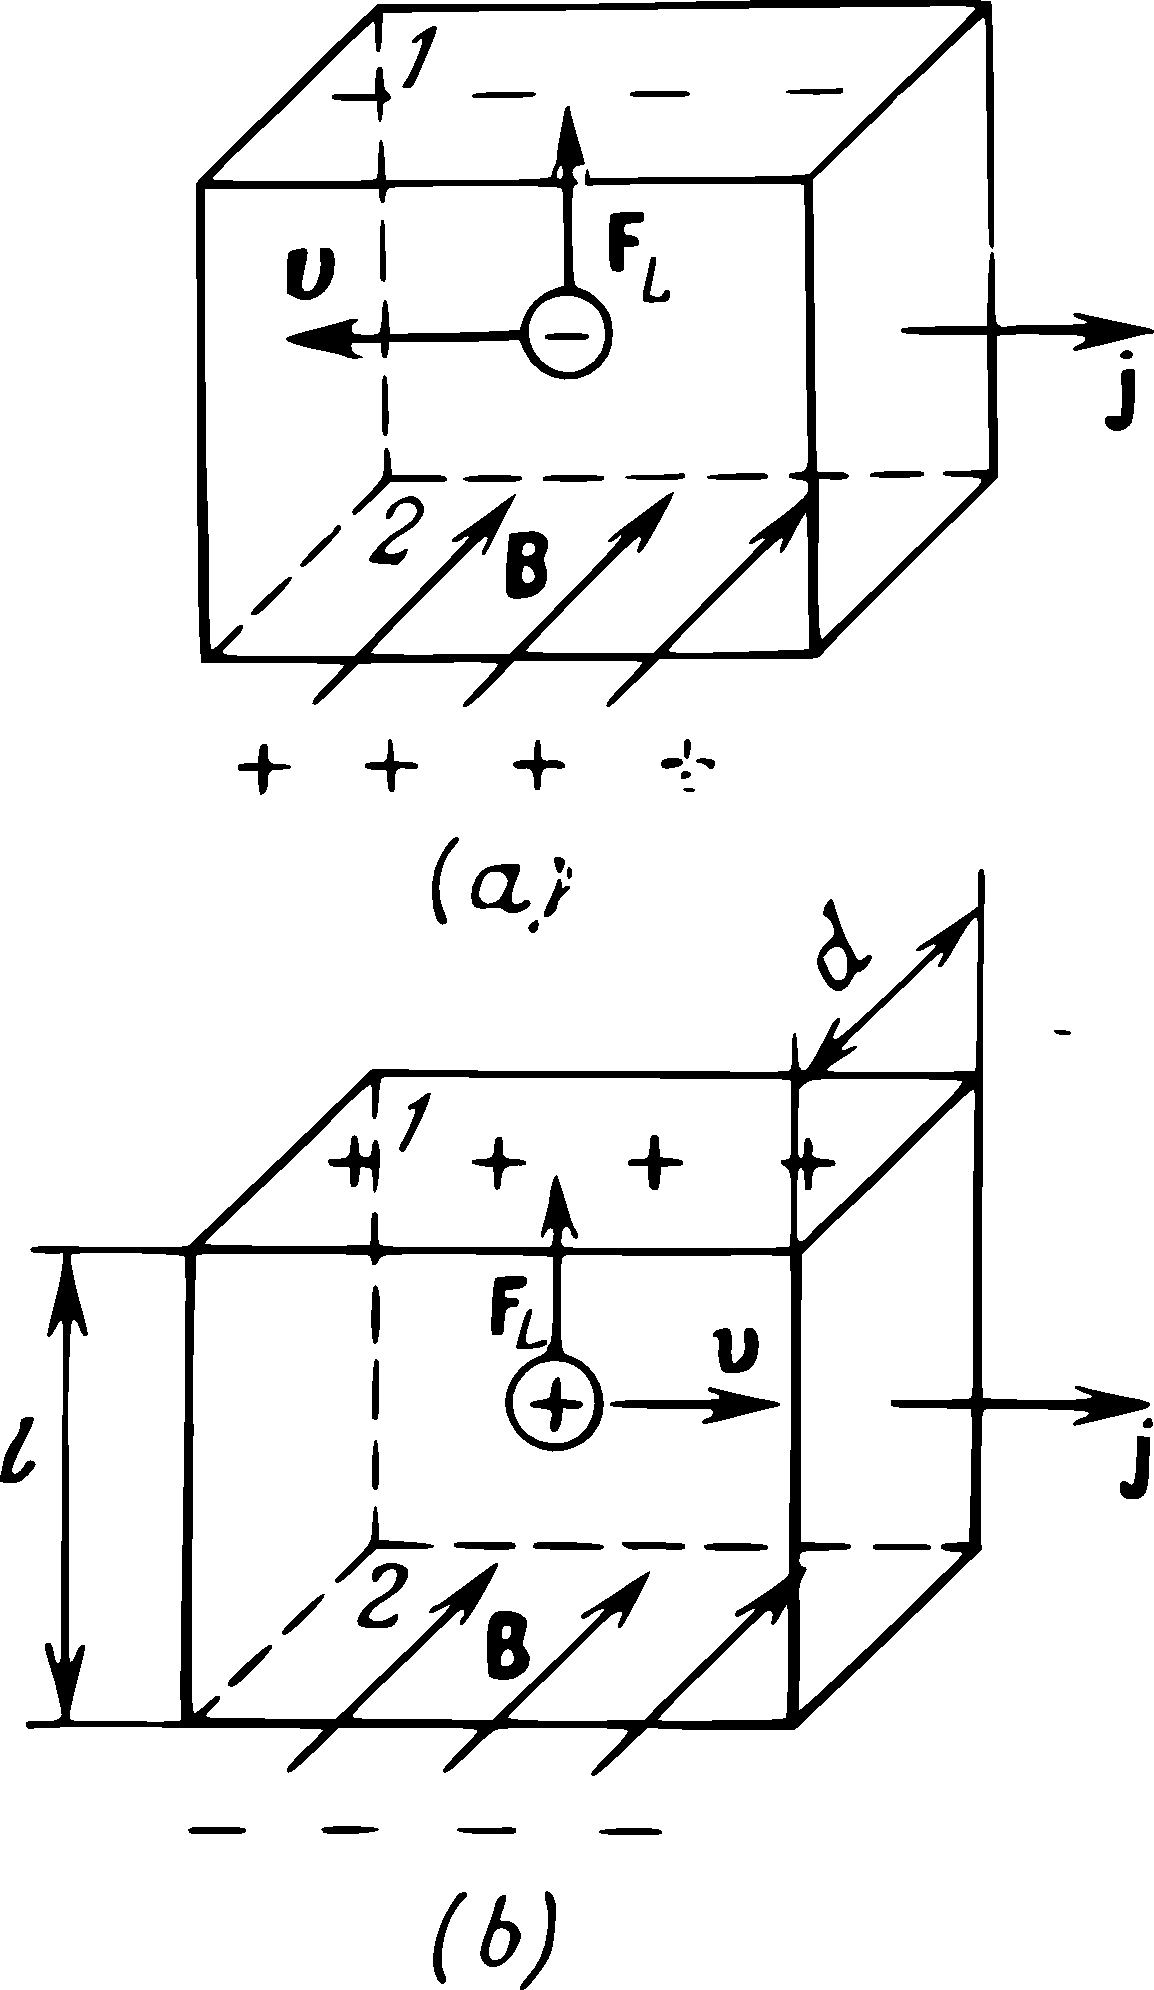
\includegraphics[width=0.8\textwidth]{figs/ch-24/fig-24-04.pdf}
\sidecaption{Path of a charged particle is a helix if the velocity vector $\vb{v}$ of a charged particle makes the angle $\alpha$ with the direction of vector $\vb{B}$ of a uniform magnetic field.\zhcap{若带电粒子的速度矢量 $\vb{v}$ 与均匀磁场的磁感应强度 $\vb{B}$ 方向成夹角 $\alpha$，则其轨迹为螺旋线。}\label{fig-24-04}}
\end{marginfigure}
If this motion occurs in a nonuniform magnetic field \ssect{23.1.3} whose magnetic induction increases in the direction of motion of the particle, then $r$ and $h$ decrease with an increase in ${B}$. This phenomenon is used for focusing charged particles in a magnetic field.
\zhpar{若该运动发生在非均匀磁场（\ssect{23.1.3}）中，且磁感应强度沿粒子运动方向增大，则 $r$ 和 $h$ 随 ${B}$ 的增大而减小。这一现象被用于磁场中带电粒子的聚焦。}

\section{Hall Effect}\label{sec-24.2}
\zhtitle{霍尔效应}




\subsection{}\label{24.2.1} The \redem{Hall effect} refers to the setting up of a transverse electric field and potential difference in a current-carrying metal or semiconductor placed in a magnetic field which is perpendicular to the direction of the current density vector \ssect{20.2.3}. The Hall effect results from the deflection of electrons moving in a magnetic field by the action of the Lorentz force \ssect{24.1.1}.
\zhpar{\redem{霍尔效应}是指：在置于磁场中、且磁场方向与电流密度矢量（\ssect{20.2.3}）垂直的载流金属或半导体中，产生横向电场和电势差。霍尔效应源于运动电子在磁场中受洛伦兹力（\ssect{24.1.1}）作用而发生的偏转。}



Shown in \figr{fig-24-04}~\drkgry{(a)} are the directions of the magnetic induction $\vb{B}$, current density $\vb{j}$, electron velocity $\vb{v}$, Lorentz force $\vb{F}_{L}$ and the signs of the charges accumulated on the opposite, upper and lower, sides in the case of a metal or electron ($n$-type) semiconductor \ssect{41.10.2}. In a hole ($p$-type) semiconductor \ssect{41.10.3} the signs of the charges on the surfaces are the opposite of those in the preceding case (\figr{fig-24-04}~\drkgry{(b)}). The charges are deflected by the magnetic field until the action of the force in the transverse electric field counterbalances the Lorentz force.
\zhpar{如\figr{fig-24-04}~\drkgry{(a)}所示，给出了磁感应强度 $\vb{B}$、电流密度 $\vb{j}$、电子速度 $\vb{v}$、洛伦兹力 $\vb{F}_{L}$ 的方向，以及在金属或电子型（$n$ 型）半导体（\ssect{41.10.2}）中位于上、下两个相对侧面的电荷符号。对于空穴型（$p$ 型）半导体（\ssect{41.10.3}），两侧面上电荷的符号与前一情形相反（见\figr{fig-24-04}~\drkgry{(b)}）。电荷在磁场作用下发生偏转，直至横向电场的作用力与洛伦兹力相互抵消为止。}

\subsection{}\label{24.2.2} The equilibrium potential difference in the Hall effect is
\zhpar{霍尔效应中的平衡电势差为：}
\begin{equation*}%
\Delta V = V_{1} - V_{2} = R_{H} \, \frac{IB}{d},
\end{equation*}
where $I$ is the current, $B$ is the magnetic field induction \ssect{23.1.2}, $d$ is the linear dimension of the metal or semiconductor in the direction of vector $\vb{B}$, and $R_{H}$ is the Hall coefficient.
\zhpar{式中 $I$ 为电流，$B$ 为磁感应强度（\ssect{23.1.2}），$d$ 为金属或半导体沿矢量 $\vb{B}$ 方向的线度，$R_{H}$ 为霍尔系数。}

The strength $\vb{E}_{H}$ of the transverse electric field in the Hall effect is
\zhpar{霍尔效应中横向电场的强度 $\vb{E}_{H}$ 为：}
\begin{equation*}%
\vb{E}_{H} = R_{H} \, [\vb{B} \cross \vb{j}],
\end{equation*}
where $\vb{j}$ is the current density vector.
\zhpar{式中 $\vb{j}$ 为电流密度矢量。}

\subsection{}\label{24.2.3} For metals and extrinsic semiconductors \ssect{41.10.5}, having a single kind of conduction, the Hall coefficient equals
\zhpar{对于只有一种导电类型的金属和杂质半导体（\ssect{41.10.5}），霍尔系数为：}
\begin{align*}%
R_{H} & = \frac{A }{n_{0}q} &&  \text{(in SI units),} \\
R_{H} & = \frac{A }{cn_{0}q} &&  \text{(in Gaussian units),}
\end{align*}
where $c$ is the electrodynamic constant \ssect{23.2.2}, $q$ and $n_{0}$ are the charge and concentration of the current carriers, and $A \approx 1$ is a dimensionless factor depending upon how the current-carrier velocities are statistically distributed. The sign of the Hall coefficient coincides with that of the current-carrier charge $q$. A measurement of the Hall coefficient of a semiconductor indicates its type of electrical conduction. For an $n$-type semi­-conductor (electron conduction) \ssect{41.10.2}, $q= -e$ and $R_{H}< 0$; for a $p$-type semiconductor (hole conduction) \ssect{41.10.3}, $q = e$ and $R_{H} > 0$.
\zhpar{式中 $c$ 为电动力学常量（\ssect{23.2.2}），$q$ 与 $n_{0}$ 分别为载流子的电荷与浓度，$A \approx 1$ 为无量纲因子，取决于载流子速度的统计分布方式。霍尔系数的符号与载流子电荷 $q$ 的符号一致。测量半导体的霍尔系数可以确定其导电类型。对于 $n$ 型半导体（电子导电，\ssect{41.10.2}），$q= -e$，$R_{H}< 0$；对于 $p$ 型半导体（空穴导电，\ssect{41.10.3}），$q = e$，$R_{H} > 0$。}

If both types of electrical conduction are observed in a semi-conductor, the predominant conduction can be determined from the sign of the Hall coefficient. The formula for $R_{H}$ given in
this subsection is inapplicable in such cases.
\zhpar{若半导体中同时存在两种导电类型，则可根据霍尔系数的符号判断占优势的导电类型。在这种情形下，本小节给出的 $R_{H}$ 公式不适用。}

\subsection{}\label{24.2.4} Provided the type of electrical conduction is known, a measurement of the Hall coefficient enables the concentration $n_{0}$ of the current carriers to be determined. For example, the concentration of conduction electrons equals the concentration of atoms in monovalent metals. This means that there is one free electron per atom in the electron gas \ssect{20.3.1} of the metal. A known concentration of current carriers enables the mean free path $\expval{\, \lambda \,}$ of the electron in the metal to be assessed. From the formula of \ssect{20.3.4},
\zhpar{在导电类型已知的情况下，测量霍尔系数可以确定载流子的浓度 $n_{0}$。例如，对于一价金属，传导电子的浓度等于原子的浓度，这意味着金属的电子气（\ssect{20.3.1}）中每个原子对应一个自由电子。已知载流子浓度后，即可估算金属中电子的平均自由程 $\expval{\, \lambda \,}$。由 \ssect{20.3.4} 中的公式，}
\begin{equation*}%
\expval{\, \lambda \,} = \frac{2 \varkappa m \expval{\, u \,}}{n_{0}e^{2}},
\end{equation*}
we find that $\expval{\, \lambda \,} \approx \SI{d-8}{\meter}$, which exceeds the lattice constants of the metal by two orders of magnitude (see also Sections \ssect{20.3.7} and \ssect{41.5.5}).
\zhpar{可得 $\expval{\, \lambda \,} \approx \SI{d-8}{\meter}$，它比金属的晶格常量大两个数量级（另见\ssect{20.3.7}和\ssect{41.5.5}）。}




\section{Charge-to-Mass Ratio of Particles. Mass
Spectroscopy}
\label{sec-24.3}
\zhtitle{粒子的荷质比。质谱学}

\subsection{}\label{24.3.1} The \redem{charge-to-mass} ratio of a particle, $q/m$, is a characteristic of charged particles. Experimental determination of this charge-to-mass ratio is based on measuring the deflection of the particles in electric and magnetic fields acting jointly on them. The mass of the particles is determined from the charge-to-mass ratio $q/m$ and the known charge $q$. 
\zhpar{粒子的\redem{荷质比}，即 $q/m$，是带电粒子的特征量。荷质比的实验测定基于测量粒子在共同作用的电场与磁场中的偏转。已知电荷 $q$ 时，可由荷质比 $q/m$ 确定粒子的质量。}

\subsection{}\label{24.3.2} The \redem{mass spectrum} of particles is the set of their mass values. Applying mass spectrometers and mass spectrographs, special instruments used in \redem{mass spectrometry}, the relative concentrations of isotopes of chemical elements \ssect{42.1.3} and their masses can be measured with exceptionally high accuracy.
\zhpar{粒子的\redem{质谱}是其质量值的集合。利用质谱仪和质谱分析仪这类专用于\redem{质谱分析}的仪器，可以极高的精度测量化学元素同位素的相对丰度（\ssect{42.1.3}）及其质量。}

\subsection{}\label{24.3.3} In the \redem{Aston mass
spectrograph} (\figr{fig-24-05}), which was employed to discover the isotopes  of various chemical elements, the particles are deflected in the uniform electric field of capacitor $C$ and the magnetic field of coil $M$, the fields being perpendicular to each other. The lower the velocity of the particles and the greater their charge-to-mass ratio, the more strongly they are deflected toward the capacitor plates. In a uniform magnetic field with the induction $\vb{B}$ directed into the drawing, the particles travel along circular arcs \ssect{24.1.6}. The higher the velocity of the particles and the lower their charge-to-mass ratio, the greater the radii of these arcs. 
\zhpar{在用于发现各种化学元素同位素的\redem{阿斯顿质谱仪}（见\figr{fig-24-05}）中，粒子在电容器 $C$ 的均匀电场和线圈 $M$ 的磁场中发生偏转，两场相互垂直。粒子的速度越小、荷质比越大，则其越强烈地偏向电容器极板。在磁感应强度为 $\vb{B}$、方向指向图面里侧的均匀磁场中，粒子沿圆弧运动（\ssect{24.1.6}）。粒子的速度越大、荷质比越小，圆弧的半径就越大。}

\begin{marginfigure}[-2cm]
\centering
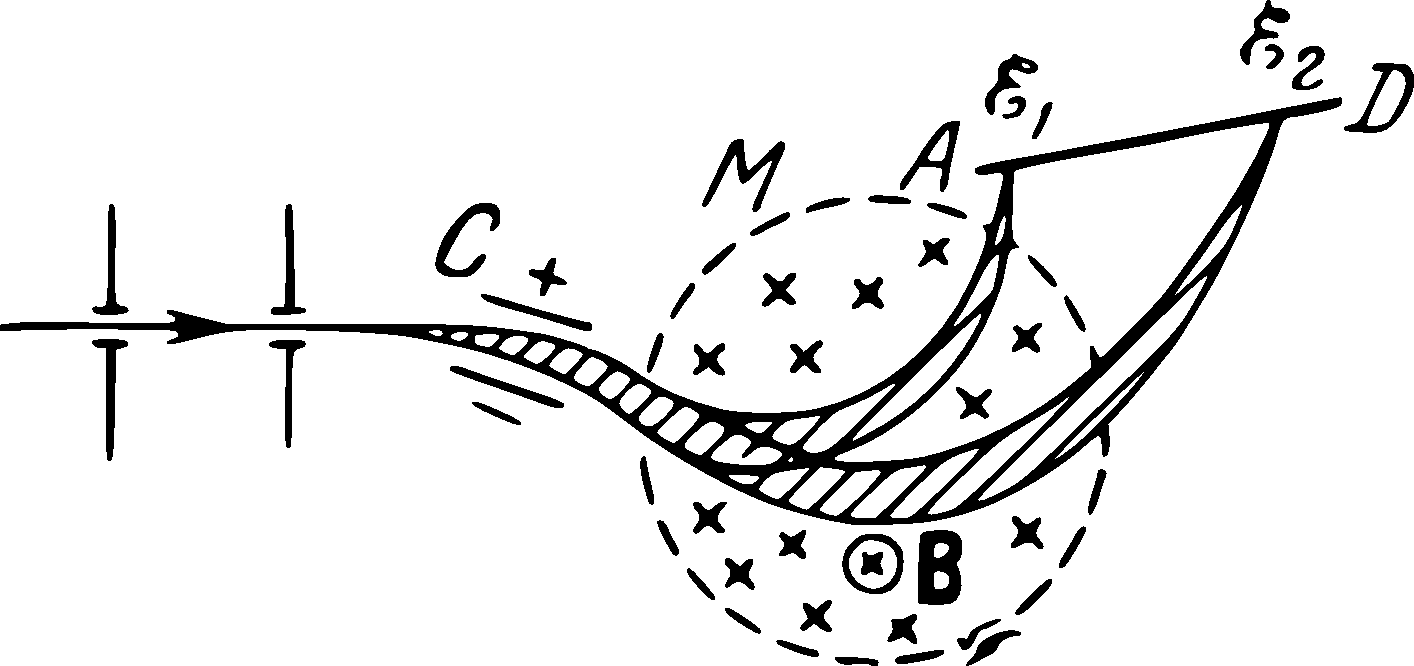
\includegraphics[width=0.8\textwidth]{figs/ch-24/fig-24-05.pdf}
\sidecaption{Schematic diagram of a Aston mass
spectrograph.\zhcap{阿斯顿质谱仪示意图。}\label{fig-24-05}}
\end{marginfigure}


In a magnetic field a beam of particles is split into several beams, each corresponding to a definite charge-to-mass ratio. The magnetic field focuses particles having different velocities, but the same charge-to-mass ratio, on a single point. The magnetic induction $\vb{B}$ is chosen so that the charged particles are focused on a photographic plate $AD$, which is perpendicular to the plane of the drawing. A series of narrow parallel lines obtained on the plate corresponds to the various values of the particle charge-to-mass ratio. In \figr{fig-24-05}, line $\emf_{1}$ corresponds to particles with a higher charge-to-mass ratio, and line $\emf_{2}$ to particles with a lower one. If the charge-to-mass ratio of the particles of line $\emf_{1}$ is known, as well as the distance between lines $\emf_{1}$ and $\emf_{1}$ and the parameters of the instrument, the charge-to-mass ratio of the particles corresponding to line $\emf_{1}$ can be determined.
\zhpar{在磁场中，粒子束被分裂为若干束，每一束对应一个确定的荷质比。磁场能够将速度不同而荷质比相同的粒子聚焦于同一点。选取磁感应强度 $\vb{B}$，使带电粒子聚焦于与图面垂直的照相底板 $AD$ 上。底板上得到的一系列细的平行线对应于粒子荷质比的各个不同数值。在\figr{fig-24-05}中，谱线 $\emf_{1}$ 对应荷质比较大的粒子，谱线 $\emf_{2}$ 对应荷质比较小的粒子。若已知谱线 $\emf_{1}$ 上粒子的荷质比，以及谱线 $\emf_{1}$ 与 $\emf_{1}$ 之间的距离和仪器参数，即可确定谱线 $\emf_{1}$ 上粒子的荷质比。}

If the parallel-plate capacitors are replaced by tubular ones and special electromagnets are used that produce a plane-parallel beam of particles entering the magnetic field, we can achieve \redem{double focusing} of the particles with respect to both energy and direction. With sufficient intensity of the lines on the photo­ graphic plate, this technique ensures high precision in particle mass measurements. For instance, the masses of the ions of light-weight elements can be measured to an accuracy within \num{d-4} per cent.
\zhpar{若将平行板电容器换成圆柱形电容器，并使用特殊的电磁铁产生使粒子以平面平行束进入磁场的条件，则可以实现粒子在能量和方向两方面的\redem{双聚焦}。若照相底板上的谱线足够清晰，这一技术可以保证质量测量的高精度。例如，轻元素离子的质量可以精确到 \num{d-4}\% 以内。}

\subsection{}\label{24.3.4} The relative concentrations of the isotopes of chemical elements in their natural mixtures are measured by instruments called \redem{mass spectrometers} that electrically record the ion currents. Used in mass spectrometers are ion beams in which the kinetic energies of the ions are close in value. These are called mono­chromatic (monoenergetic) beams and are produced by ion sources of special design. Even when they are strongly divergent and contain a great number of ions, such beams focus well in a transverse magnetic field. This raises the precision with which the concentrations of various isotopes can be measured.
\zhpar{化学元素同位素在天然混合物中的相对丰度，由称为\redem{质谱仪}的仪器测量，该仪器以电学方法记录离子流。质谱仪中使用的是离子动能数值相近的离子束，这种离子束称为\redem{单能离子束}，由专门设计的离子源产生。即使这些离子束发散程度很大、所含离子数目很多，它们在横向磁场中仍能很好地聚焦。这提高了测量各种同位素浓度的精度。}

\section{Charged Particle Accelerators}
\label{sec-24.4}
\zhtitle{带电粒子加速器}

\subsection{}\label{24.4.1} Special installations for obtaining directed beams of charged particles (electrons, protons, atomic nuclei and ions of chemical elements) having an extremely high kinetic energy, under laboratory conditions are called \redem{accelerators}. According to the shape of the path of the particles and the mechanism for accelerating them, distinction is made between \redem{linear}, \redem{cyclic} and \redem{induction accelerators}. In linear accelerators (also called \redem{linacs}) the paths of motion of the particles are close to straight lines; in the cyclic and induction accelerators the paths of the particles are circles or unwinding spirals.
\zhpar{能够在实验室条件下获得动能极高的定向带电粒子束（电子、质子、原子核以及化学元素的离子）的装置，称为\redem{加速器}。根据粒子的运动轨道形状及加速机制，可分为\redem{直线}、\redem{循环}和\redem{感应}加速器。在直线加速器（亦称 linac）中，粒子的运动轨迹接近直线；在循环加速器和感应加速器中，粒子的轨迹为圆或展开的螺旋线。}

\subsection{}\label{24.4.2} The energy of the accelerated particles is increased by the electric field set up in the accelerator. Depending on the type of accelerator, this field can be electrostatic \ssect{15.1.2}, induced \ssect{25.1.2} or high-frequency alternating. The principle of the betatron, based on the action of an induced electric field, is discussed in section \ssect{27.2.3}. In a \redem{linear electrostatic accelerator}, a charged particle passes only once through an accelerating electric field with a potential difference $(V_{1} - V_{2})$. If $q$ is the charge of the particle, the energy acquired by the particle in the accelerator \ssect{16.2.7} is equal to
\zhpar{粒子获得的能量由加速器中建立的电场提供。根据加速器类型的不同，该电场可以是静电场（\ssect{15.1.2}）、感生电场（\ssect{25.1.2}）或高频交变电场。基于感生电场作用的电子感应加速器（betatron）的原理在 \ssect{27.2.3} 中讨论。在\redem{直线静电加速器}中，带电粒子只通过一次电势差为 $(V_{1} - V_{2})$ 的加速电场。若 $q$ 为粒子的电荷，则粒子在加速器中获得的能量（\ssect{16.2.7}）为：}
\begin{equation*}%
E = q(V_{1} - V_{2}).
\end{equation*}
In such an accelerator the electric field is set up, for example, by a \redem{Van de Graaff} high-voltage \redem{electrostatic generator}, operating by the principle of multiple transfer of charges to a hollow conductor \ssect{16.4.3}. This raises the potential of the conductor to values limited only by the leakage of the charge from the conductor.
\zhpar{在这种加速器中，电场可由例如\redem{范德格拉夫}高压\redem{静电发生器}建立，其工作原理是将电荷多次转移到空心导体上（\ssect{16.4.3}）。这使导体的电势升高，其数值仅受导体上电荷泄漏的限制。}

\subsection{}\label{24.4.3} In \redem{linear resonant accelerators}, the energy of the charged particles is increased by an alternating electric field of super-high frequency, which varies in synchronism with the motion of the particles. Using this type of accelerator, electrons can be accelerated to an energy of the order of dozens of \si{\giga\electronvolt} over a path length of several kilometres.
\zhpar{在\redem{直线共振加速器}中，粒子的能量由超高频交变电场增加，该电场的变化与粒子的运动同步。利用这种加速器，可以在长度为数千米的路径上将电子加速到数十 \si{\giga\electronvolt} 量级的能量。}

\subsection{}\label{24.4.4} Protons, deuterons and other, heavier, charged particles are accelerated by \redem{resonant cyclic accelerators}, in which a particle repeatedly passes through an electric field synchronized with its motion, increasing its energy each time. A strong transverse magnetic field controls the motion of the particles and returns them periodically to the region of the accelerating electric field. The particles pass definite points of the alternating electric field approximately when the field is in the same phase (``in resonance'').
\zhpar{质子、氘核以及其他较重的带电粒子由\redem{共振循环加速器}加速。在这种加速器中，粒子反复通过与其运动同步的电场，每次通过都使能量增加。强横向磁场控制粒子的运动，并使其周期性地回到加速电场区域。粒子通过交变电场中的确定点时，电场大致处于相同的相位（即“共振”）。}

\subsection{}\label{24.4.5} In the \redem{cyclotron}, the simplest resonant cyclic accelerator, an accelerating alternating electric field is set up in the gap between the two halves (\redem{dees}) $N$ and $M$ (\figr{fig-24-06}) of a cylindrical box. The dees are placed in a flat closed chamber located between the poles of a strong electromagnet, whose magnetic field is perpendicular to the plane of the drawing. The alternating electric field in the gap between the dees is set up by an electric generator whose terminals are connected to electrodes $m$ and $n$.
\zhpar{\redem{回旋加速器}是最简单的共振循环加速器，其加速交变电场建立在圆柱形盒子的两个半盒（\redem{D形盒}）$N$ 与 $M$ 之间的间隙中（见\figr{fig-24-06}）。D形盒置于强电磁铁两极之间的扁平密封腔室内，磁场与图面垂直。D形盒间隙中的交变电场由发电机产生，发电机的端子与电极 $m$ 和 $n$ 相连。}

\begin{marginfigure}%[-2cm]
\centering
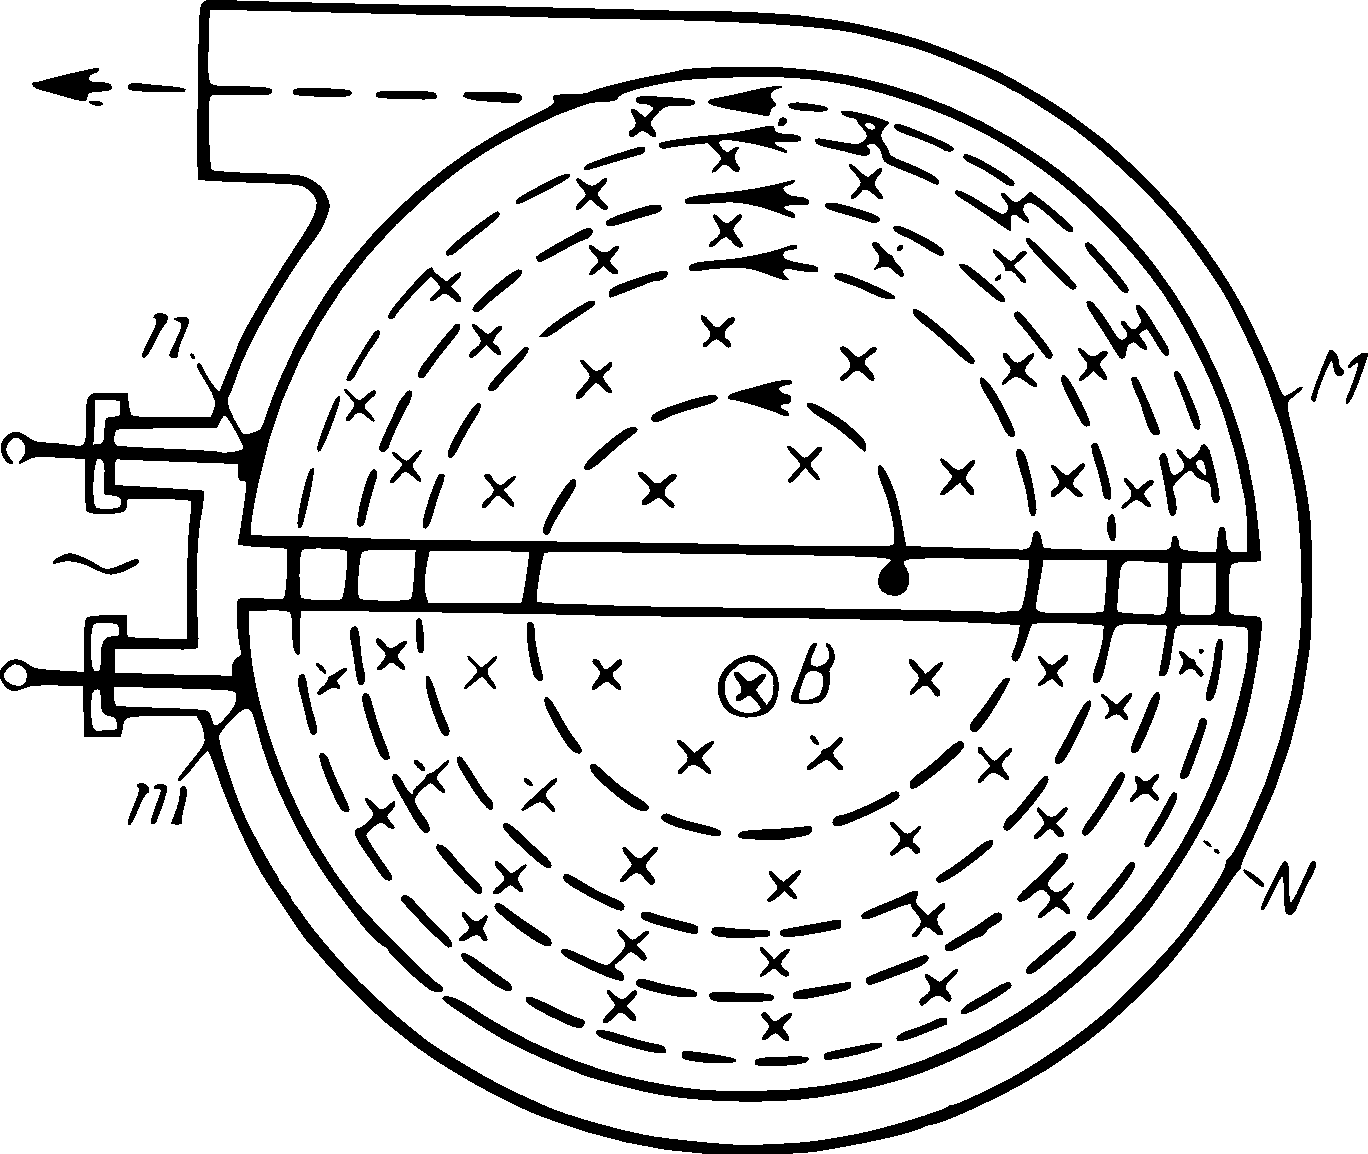
\includegraphics[width=0.9\textwidth]{figs/ch-24/fig-24-06.pdf}
\sidecaption{Schematic diagram of a cyclotron.\zhcap{回旋加速器示意图。}\label{fig-24-06}}
\end{marginfigure}



\subsection{}\label{24.4.6} A particle is accelerated in the gap between the dees $M$ and $N$ each time it crosses this gap after describing semicircles of continuously increasing radii due to the action of the magnetic field. The same time is required for each semicircle \ssect{24.1.6}. To continuously accelerate the particles it is necessary to com­ ply with the condition of synchronism (condition of ``resonance''): $T = T_{0}$, where $T$ is the period of revolution of the particle in the magnetic field \ssect{24.1.6}, and is the period of oscillation of the magnetic field \ssect{28.1.2}. This condition is violated at rel­ativistic velocities $v$ of the particle, commensurate with the velocity of light $c$ in free space. At such high velocities, the mass $m$ of the particle increases with the velocity \ssect{5.6.1} as does the period $T$ \ssect{24.1.6}.
\zhpar{粒子每次穿过 D形盒 $M$ 与 $N$ 之间的间隙时都会被加速，同时在磁场作用下，粒子沿半径不断增大的半圆轨道运动。每个半圆所需的时间相同（\ssect{24.1.6}）。为了使粒子持续被加速，必须满足同步条件（即“共振条件”）：$T = T_{0}$，其中 $T$ 是粒子在磁场中的回旋周期（\ssect{24.1.6}），$T_{0}$ 是交变电场的振荡周期（\ssect{28.1.2}）。当粒子的速度 $v$ 与真空中的光速 $c$ 相当、达到相对论速度时，该条件即被破坏。在如此高的速度下，粒子的质量 $m$ 随速度增大（\ssect{5.6.1}），其周期 $T$ 也随之增大（\ssect{24.1.6}）。}

\subsection{}\label{24.4.7} The feasibility of accelerating charged particles travelling at relativistic velocities in cyclic accelerators follows from the \redem{principle of phase stability} (\redem{autophasing}), which states that each deviation of the period $T$ from the resonance value $T_{0}$ \ssect{24.4.6} leads to such a change in the energy $E$ of the particle at each acceleration that $T$ varies in the neighborhood of $T_{0}$ and, on an average, remains equal to $T_{0}$. Thus
\zhpar{相对论速度下的带电粒子在循环加速器中被加速的可行性，源于\redem{相稳定性原理}（\redem{自动同相}）。该原理指出：周期 $T$ 对共振值 $T_{0}$（\ssect{24.4.6}）的每一次偏离，都会使粒子在每次加速时的能量 $E$ 发生相应改变，从而使 $T$ 在 $T_{0}$ 附近变化，并且平均而言仍等于 $T_{0}$。于是有：}
\begin{equation*}%
T_{0} \approx T = \frac{2\pi}{B} \, \frac{m}{\abs{q}} = \frac{2 \pi}{B} \, \frac{E}{\abs{q} c^{2}},
\end{equation*}
where $E = mc^{2}$ \ssect{5.7.2}, $m = m_{0}/\sqrt{ 1 - v^{2}/c^{2}}$ \ssect{5.6.1}, $m_{0}$ is the rest mass \ssect{5.6.1} of the particle, and $c$ is the velocity of light in free space; the remaining notation is the same as in section \ssect{24.1.6}.
\zhpar{式中 $E = mc^{2}$（\ssect{5.7.2}），$m = m_{0}/\sqrt{ 1 - v^{2}/c^{2}}$（\ssect{5.6.1}），$m_{0}$ 为粒子的静止质量（\ssect{5.6.1}），$c$ 为真空中的光速；其余符号与 \ssect{24.1.6} 中的相同。}

If, for example, as a result of the increase in mass $m$ and the period $T$, the particle enters the gap between the dees (\figr{fig-24-06}) by the action of the decelerating instead of accelerating electric field, the reduction in particle velocity leads to the reduction in $T$ and the equality $T = T_{0}$ is reached again.
\zhpar{例如，由于质量 $m$ 和周期 $T$ 的增大，粒子进入D形盒间隙时所受的电场为减速电场而非加速电场（见\figr{fig-24-06}），粒子速度的减小会使 $T$ 减小，从而重新达到 $T = T_{0}$ 的条件。}

\subsection{}\label{24.4.8} It follows from the principle of phase stability \ssect{24.4.7} that at a sufficiently slow increase in the period $T_{0}$ of the elec­tric field, the period $T$ of revolution of the particle in the magnetic field of the accelerator increases correspondingly. This leads to an increase in the average energy $\expval{E}$ of all the particles because at constant induction of the magnetic field any increase in $T$ is possible only owing to the increase in mass as the velocity of the particles increases.
\zhpar{由相稳定性原理（\ssect{24.4.7}）可知，若电场的周期 $T_{0}$ 足够缓慢地增大，则粒子在加速器磁场中的回旋周期 $T$ 也相应增大。由于磁感应强度恒定，$T$ 的任何增大都只能是粒子速度增大、质量随之增大的结果，因此所有粒子的平均能量 $\expval{E}$ 随之增大。}

This principle has been applied in an accelerator called the \redem{synchrocyclotron} (also \redem{frequency-modulated cyclotron} and \redem{phasotron}). This device has a constant magnetic field, whereas the frequency $\nu_{0}= 1/T_{0}$ \ssect{28.1.2} of the alternating electric field varies slowly with the period $\tau \gg T_{0}$. The radius of the orbit of the particles in the synchrocyclotron increases with their velocity \ssect{24.1.6}. This requires a corresponding increase in the size of the synchrocyclotron to reach the maximum energy of the charged particles. The synchrocyclotron built and operated in the USSR, accelerating protons to an energy of \SI{680}{\mega\electronvolt},
has a magnet with poles \SI{6}{\meter} in diameter and a mass of \SI{7d6}{\kilo\gram}.
\zhpar{这一原理已应用于一种称为\redem{同步回旋加速器}（亦称\redem{调频回旋加速器}和\redem{调相加速器}）的加速器中。该装置的磁场恒定，而交变电场的频率 $\nu_{0}= 1/T_{0}$（\ssect{28.1.2}）以周期 $\tau \gg T_{0}$ 缓慢变化。同步回旋加速器中粒子轨道的半径随粒子速度增大而增大（\ssect{24.1.6}），因此要达到带电粒子的最大能量，需要相应增大同步回旋加速器的尺寸。苏联建成并运行的一台同步回旋加速器，可将质子加速到 \SI{680}{\mega\electronvolt} 的能量，其磁极直径为 \SI{6}{\meter}，磁铁质量为 \SI{7d6}{\kilo\gram}。}

\subsection{}\label{24.4.9} The \redem{synchrotron} is an accelerator in which the frequency of the accelerating electric field is constant, and the induction $B$ of the magnetic field varies with time. The period of revolution of a particle in the magnetic field of a synchrotron \ssect{24.4.6} is
\zhpar{\redem{同步加速器}是一种加速电场频率恒定、而磁感应强度 $B$ 随时间变化的加速器。同步加速器中粒子在磁场中的回旋周期（\ssect{24.4.6}）为：}
\begin{equation*}%
T = \frac{2\pi}{\abs{e}c^{2}} \, \frac{E}{B},
\end{equation*}
where $e$ is the charge of the electron, and $E$ is its energy. The condition of synchronism \ssect{24.4.6} is complied with in a synchrotron at $T_{0} = \text{const.}$, provided that the induction of the magnetic field increases proportionally to the particle's energy. Thus
\zhpar{式中 $e$ 为电子的电荷，$E$ 为其能量。在同步加速器中，只要磁感应强度随粒子能量成正比增大，即可在 $T_{0} = \text{const.}$ 的条件下满足同步条件（\ssect{24.4.6}）。于是有：}
\begin{equation*}%
B = \frac{2\pi}{\abs{e}c^{2}} \, \frac{E}{T_{0}},
\end{equation*}
where $T_{0}$ is the period of a high-frequency accelerating electric field.
\zhpar{式中 $T_{0}$ 为高频加速电场的周期。}

The following condition is complied with in a synchrotron:
\zhpar{同步加速器中满足如下条件：}
\begin{equation*}%
\frac{m}{B} = \frac{eT_{0}}{2 \pi} = \text{const.}
\end{equation*}
The particles travel along orbits close to circular ones \ssect{24.1.6} and, consequently, a synchrotron is equipped with annular magnets that set up a magnetic field in a comparatively narrow region of the circular orbit.
\zhpar{粒子沿近似圆形的轨道运动（\ssect{24.1.6}），因此同步加速器配有环形磁铁，用以在圆轨道的较窄区域内建立磁场。}

\subsection{}\label{24.4.10} A \redem{proton synchrotron}, the most powerful accelerator of protons, combines the principles applied in the synchrocyclotron \ssect{24.4.8} and in the synchrotron \ssect{24.4.9}. In this accelerator, the frequency $\nu_{0}$ of the accelerating electric field is reduced and the induction $B$ of the magnetic held is increased simultaneously and in coordination. The protons being accelerated travel along a circular orbit of constant radius. Therefore, the magnetic field is set up by an annular electromagnet as in the synchrotron.
\zhpar{\redem{质子同步加速器}是最强大的质子加速器，它结合了同步回旋加速器（\ssect{24.4.8}）与同步加速器（\ssect{24.4.9}）的原理。在该加速器中，加速电场的频率 $\nu_{0}$ 减小，同时磁场的磁感应强度 $B$ 增大，二者协调一致地同时变化。被加速的质子沿半径恒定的圆轨道运动，因此与同步加速器一样，磁场由环形电磁铁建立。}

\subsection{}\label{24.4.11} The condition for simultaneous maintenance of vertical (axial) and radial stability of the design circular orbit in the synchrotron and proton synchrotron is the variation of magnetic induction $B$ near the design orbit according to the law
\zhpar{要使同步加速器和质子同步加速器中的设计圆轨道同时具有竖直（轴向）稳定性和径向稳定性，设计轨道附近的磁感应强度 $B$ 须按如下规律变化：}
\begin{equation*}%
B = \frac{\text{const.}}{r^{n}},
\end{equation*}
where $r$ is the distance from the centre of the orbit, and $n$ varies within the limits $0 < n < 1$ (\redem{condition of weak focusing} in the accelerator). With an increase in the maximum energy $E_{\text{max}}$ acquired by the particles in an accelerator having weak focusing, the required mass of the electromagnet increases approximately in proportion to $E_{\text{max}}^{3}$.
\zhpar{式中 $r$ 为离开轨道中心的距离，$n$ 在 $0 < n < 1$ 范围内取值（加速器中的\redem{弱聚焦条件}）。随着弱聚焦加速器中粒子所获得的最大能量 $E_{\text{max}}$ 增大，所需电磁铁的质量大致与 $E_{\text{max}}^{3}$ 成正比增加。}

\subsection{}\label{24.4.12} Accelerators having \redem{strong focusing} are resorted to for increasing the maximum energy $E_{\text{max}}$ of particles accelerated in synchrotrons and proton synchrotrons. In these accelerators, two kinds of sector-shaped magnets are used alternately along the almost circular orbit of particle travel. In one kind of sector the magnetic field varies according to the law of section \ssect{24.4.11}, in which $n$ is much less than zero (for example, $n = - 100$), and in the other kind $n \gg 1$. Sectors of the first type provide for radial focusing of the beam of particles being accelerated; sectors of the second kind, for vertical focusing. The application of strong focusing enables substantial reductions to be obtained in the overall size of the accelerator, the mass of the electromagnet and the total cost of the installation. This method is also called alternating-gradient focusing.
\zhpar{为了提高同步加速器和质子同步加速器中粒子所能获得的最大能量 $E_{\text{max}}$，采用了\redem{强聚焦}加速器。在这种加速器中，沿粒子运动的近似圆形轨道交替使用两种扇形磁铁。在一种扇形区中，磁场按 \ssect{24.4.11} 中的规律变化，其中 $n$ 远小于零（例如 $n = - 100$）；在另一种扇形区中，$n \gg 1$。第一类扇形区提供被加速粒子束的径向聚焦，第二类扇形区提供竖直聚焦。采用强聚焦可以显著减小加速器的总尺寸、电磁铁的质量以及整套装置的总造价。这种方法也称为交变梯度聚焦。}

\subsection{}\label{24.4.13} To increase the share of energy utilized by accelerated particles for various nuclear reactions \ssect{42.9.1}, the bombardment of stationary targets by high-energy particles is replaced by the \redem{colliding beam technique}. It follows from the laws of conservation of energy \ssect{3.4.3} and momentum \ssect{2.7.1} that in bombarding a stationary target, the share of the kinetic energy $E_{k}$ of the incident particle, utilized in the nuclear reaction, decreases as $E_{k}$ is increased. When the technique of colliding beams is used, the total momentum of the particles after collision is reduced and the share of their useful energy is increased. Assume, for example, that in an accelerator with colliding beams of protons the energy of the protons in each beam is equal to \SI{26}{\giga\electronvolt}. The total momentum of two protons colliding at equal and opposing velocities equals zero. But the collision energy of such two particles reaches \SI{50}{\giga\electronvolt}. To obtain the same collision energy in bombarding a stationary hydrogen target, a beam of protons with energy of the order of \SI{1400}{\giga\electronvolt} is required.
\zhpar{为了提高粒子加速后用于各种核反应（\ssect{42.9.1}）的能量利用率，用高能粒子轰击静止靶的做法已被\redem{对撞束技术}取代。由能量守恒定律（\ssect{3.4.3}）和动量守恒定律（\ssect{2.7.1}）可知，在轰击静止靶时，入射粒子用于核反应的动能 $E_{k}$ 所占的比例，随 $E_{k}$ 的增大而减小。采用对撞束技术时，粒子碰撞后的总动量减小，有用能量所占的比例随之增大。例如，设在质子对撞加速器中，每束质子的能量均为 \SI{26}{\giga\electronvolt}。两个以大小相等、方向相反的速度相撞的质子，其总动量为零，但它们的碰撞能量可达 \SI{50}{\giga\electronvolt}。若要用静止的氢靶获得相同的碰撞能量，则需要能量约为 \SI{1400}{\giga\electronvolt} 的质子束。}



